\documentclass[12pt,letterpaper,onecolumn]{article} %% one column, submission layout
\usepackage{col}
\usepackage[draft]{hyperref}
\usepackage{amsmath,amssymb,graphicx}
\usepackage{CJK}
\usepackage{epstopdf}
\newcommand{\rmnum}[1]{\romannumeral #1}
\newcommand{\Rmnum}[1]{\MakeUppercase{\romannumeral #1}}
\newcommand{\vect}[1]{\overline {#1}}
\newcommand{\vm}[1]{{\bf{#1}}}
\newcommand{\argmin}{\operatornamewithlimits{argmin}}
\newcommand{\argmax}{\operatornamewithlimits{argmax}}
\newcommand{\idxmin}{\operatornamewithlimits{idxmin}}
\newcommand{\idxmax}{\operatornamewithlimits{idxmax}}
\newcommand{\twopartdef}[4]
{
	\left\{
		\begin{array}{ll}
			#1 &; #2 \\
			#3 &; #4
		\end{array}
	\right.
}

\begin{document}

\title{Sample Indexed Spatial Orthogonal Frequency Division Multiplexing}

\renewcommand{\baselinestretch}{0.9}
\begin{center}
\begin{CJK*}{GBK}{kai}
\author{Pankil Butala $^{1,*}$, Hany Elgala $^1$,  and Thomas DC Little $^1$\\}
\end{CJK*}
\end{center}
\address{
\emph{$^1$\emph{Department of Electrical and Computer Engineering,\\ Boston University, Boston, MA 02215, USA\\}}
$^*$\emph{Corresponding author: pbutala@bu.edu}
}
\begin{abstract} 
Optical spatial modulation (OSM) is a multiple-transmitter technique that can provide higher data rates with low system complexity as compared to single-input single-output (SISO) systems. Orthogonal frequency division multiplexing (OFDM) is widely implemented to achieve better spectral efficiency in wireless channels. Asymmetrically clipped optical OFDM (ACO-OFDM) and DC-biased optical OFDM (DCO-OFDM) are two well-known optical OFDM (O-OFDM) techniques suitable for intensity-modulation direct-detection (IM/DD) optical systems. In this work, sample indexed spatial OFDM (SIS-OFDM) is proposed to combine OSM and O-OFDM in a novel way and achieve significant performance gain. By assigning time-domain samples of the O-OFDM transmit symbol to different transmitters, SIS-OFDM achieves much better spectral efficiency and reduced computational complexity at the transmitter as compared to previous work that combines OSM with O-OFDM in the frequency-domain. We also consider the impact of optical source biasing on overall performance, and the relative performance of imaging (ImR) versus non-imaging receiver (NImR) design for our proposed SIS-OFDM technique. Results indicate that for a $N_{tx}\times N_{rx}$ MIMO configuration where $N_{tx}=N_{rx}=4$, SIS-OFDM using ImR can achieve up to 110dB of signal-to-noise ratio (SNR) gain over comparable system using a NImR. Also, using $N_{sc}$ number of O-OFDM subcarriers provides up to $N_{sc}\times log_2(N_{tx})$ additional bits per symbol of spectral efficiency over techniques that combine OSM and O-OFDM in the frequency domain.
\end{abstract} 

%\vspace{-0.1in}
\ocis{060.4080, 060.4230, 060.4510, 060.2605.}

\maketitle %% required
% Paper Body
Recently, the increase in use of portable computing devices has created an intense demand for wireless data access. Spectral allocations and regulations limit our ability to increase the capacity of existing channels within the radio frequency (RF) spectrum. Advances made in the solid-state lighting industry are driving significant deployments of energy-efficient light emitting diode (LED) based luminaries. This has created an opportunity to use such luminaries to establish high capacity indoor visible light communication (VLC) links and reduce the bottleneck on existing RF wireless channels. Under this model, luminaries simultaneously support illumination and wireless data transmission \cite{elg11a}. OSM and O-OFDM are two techniques that have been proposed to implement such a dual-use VLC channel.

OSM is a multiple-transmitter technique in which information is encoded over (a) index of luminiares that are spatially separated and (b) modulation scheme overlayed on indexed luminaire \cite{mes10a}. Within a symbol period, only one luminaire emits a radiant flux while all other luminaires are idle. This minimizes the inter-channel interference (ICI) thus simplifying the detection process and the overall system complexity as compared to spatial multiplexing (SMP). In OSM, the bit-stream to be transmitted is divided into contiguous sections of $k=log_2(N_{tx})$ spatial bit-stream and $m=log_2(M)$ modulation bit-stream where $N_{tx}$ is the number of luminaires and $M$ is the modulation order. The $k$ bits select the luminaire to be activated while the $m$ bits select the M-ary modulation symbol to be transmitted. Thus, OSM system provides $log_2(MN_{tx})$ bits per symbol. In \cite{fat11a}, an OSM system with pulse amplitude modulation (PAM) as the overlayed modulation scheme is proposed. Reference \cite{pop12a} proposes a scheme that combines OSM with pulse position modulation (PPM) to benefit from the energy efficiency of PPM as compared to PAM. Reference \cite{but14a} shows ImR can provide significant SNR gains for OSM and SMP as compared to NImR.

\begin{figure}[!t]
\makebox[\textwidth]{\framebox[6.6in]{\rule{0pt}{2.41in}}}
\caption{Block diagram of system implementing SIS-OFDM}
	\label{figBlockDiagram}
\end{figure}

Implementation and performance comparisons of ACO-OFDM and DCO-OFDM is shown in reference \cite{mes11a}. In ACO-OFDM, data is assigned only on odd subcarriers while in DCO-OFDM all odd and even subcarriers are assigned data. Hermetian symmetry is enforced across the frequency-domain O-OFDM symbol. An inverse fast fourier transform (IFFT) process then results in a real-valued time domain signal that multiplexes the streams before transmission over the channel. In IM/DD systems, the signal is transmitted by varying the output flux from the transmitter. Thus, the transmitted signal must be non-negative and real valued. The ACO-OFDM signal can be clipped at values below zero because the resulting clipping noise is shown to be orthogonal to the signal \cite{arm06a}. Conversely, in DCO-OFDM an offset must be added to the multiplexed signal in order to minimize errors due to clipping of negative valued signal. O-OFDM achieves high spectral efficiency by enabling parallel transmission of higher order modulation symbols on orthogonal subcarriers. The number of data-subcarriers, $N_{sc}^d$, equals ($N_{sc}/4$) for ACO-OFDM and ($N_{sc}/2-1$) for DCO-OFDM where $N_{sc}$ is the total number of subcarriers. Thus the number of transmitted bits per O-OFDM symbol is given by $R^{m}=N_{sc}^d\times log_2(M)$.

An approach to combine OSM and traditional OFDM is proposed in reference \cite{gan06a}. This approach is adapted for IM/DD communications in reference \cite{zha12a}. Here, an incoming bit-stream is divided into O-OFDM and OSM streams. Data from O-OFDM stream is assigned to different subcarriers to form the frequency domain O-OFDM symbol. OSM is then implemented in the frequency domain where each data-subcarrier is assigned to a transmitter determined by the spatial bit-stream. An IFFT operation is implemented at each transmitter to multiplex the data before transmission. Spectral efficiency of this scheme is then proportional to the number of data-subcarriers. In comparison, the spectral efficiency of SIS-OFDM is proportional to the number of subcarriers which is equal to at least double the number of data-subcarriers. Additionally, the SIS-OFDM system requires a single IFFT operation, independent of the number of transmitters and thus maintains a computational complexity equal to that of SISO OFDM transmission. Finally, SIS-OFDM using an ImR achieves much better power efficiency as compared to equivalent system using NImR.

\figurename{\ref{figBlockDiagram}} illustrates the information source block diagram of a system implementing SIS-OFDM. The information source generates the input data-stream. The coder converts the data-stream into a binary bit-stream $\vm{D}$ which is divided into consecutive segments of $R^{ms}=R^{m}+R^{s}$ bits where $R^{s}=N_{sc}\times k=N_{sc}\times log_2(N_{tx})$ is the number of spatial bits . Let the $l^{th}$ such segment be denoted by $\vm{D}_l$. The first $R^{m}$ bits of $\vm{D}_l$ are collected in a vector $\vm{D}_l^m$ are are mapped by an M-QAM modulator. The generated QAM symbols are then assigned to subcarriers (based on the O-OFDM signal format, \textit{i.e.} DCO-OFDM or ACO-OFDM) to generate a frequency-domain O-OFDM symbol $\vm{X}_l^f$ of length $N_{sc}$. An IFFT operation is applied on $\vm{X}_l^f$ to produce a real-valued bipolar time-domain O-OFDM symbol $\vm{X}_l^t$ of the same length $N_{sc}$. The latter $R^{s}$ bits of $\vm{D}_l$ are collected in a vector $D_l^s$ and are mapped to $N_{sc}$ length transmitter index vector denoted by $\vm{X}_l^s$. Let $\vm{X}_l^m$ denote the real unipolar baseband signal after clipping and/or biasing, and $0\leq n_l\leq (N_{sc}-1)$ indicate the relative time index for the next SIS-OFDM symbol to be transmitted. At each time instance, an O-OFDM signal value from $\vm{X}_l^m$ is transmitted from a different luminaire indexed by $\vm{X}_l^s$. Let $\vm{X}_{n_l}$ be this $N_{tx}$ length transmission vector at time instant $n_l$. Thus the $j^{th}$ element of this vector is then given by
\begin{equation}
	\label{eqX}
	\vm{X}_{n_l}(j) = \twopartdef{\vm{X}_l^m(n_l)}{j=\vm{X}_l^s(n_l)}{0}{\text{else}}
\end{equation}

The SIS-OFDM symbol and transmit vector generation is explained using the following example which considers ACO-OFDM with $N_{sc}=8$, 4-QAM subcarrier modulation and $N_{tx}=2$. Here, $R^{m}=4$ and $R^{s}=8$, \textit{i.e} $R^{ms}=4+8=12$ bits per SIS-OFDM symbol. The assumed bits forming one SIS-OFDM symbol $\vm{D}_l$ are shown in Table \ref{tabExBits}. Table \ref{tabExample} then illustrates the data to subcarrier and transmitter index assignments. In this example, the transmitters would jointly transmit vector $\vm{X}_{n_l}=[0$ $\sqrt{2}]^T$ at relative time index $n_l=2$.
\begin{table}[b]
\makebox[\textwidth]{\framebox[3in]{\rule{0pt}{1in}}}
\caption{Example SIS-OFDM data streams using ACO-OFDM}
	%\label{tabExBits}
%\end {table}
\quad
%\begin{table}[b]
\makebox[\textwidth]{\framebox[5in]{\rule{0pt}{2in}}}
\caption{Example subcarrier and luminaire assignment}
	%\label{tabExample}
\end {table}

The indoor optical MIMO channel is modeled as,
\begin{equation}
	\label{eqChannel}
	\vm{Y}_{n_l} = \vm{H}\vm{X}_{n_l} + \vm{W}_{n_l}
\end{equation}
where $\vm{X}_{n_l}$ is the instantaneous transmit vector. $\vm{H}$ is the channel matrix and can be computed as in \cite{but13a}. $\vm{Y}_{n_l}$ is the received signal vector and $\vm{W}_{n_l}$ is zero-mean additive white gaussian noise (AWGN) vector.

The receiver can be configured such that $\vm{H}$ is of rank $N_{tx}$. In that case, $(\vm{H}^{*}\vm{H})^{-1}$ exists. The least squares estimate of transmitted vector $\vm{X}_{n_l}$ can be computed as
\begin{equation}
	\label{eqXls}
	\hat{\vm{X}}_{n_l} = (\vm{H}^{*}\vm{H})^{-1}\vm{H}^{*}\vm{Y}_{n_l}
\end{equation}

In SIS-OFDM, only one luminaire emits radiant flux at a given time instance. Thus the maximum element of $\hat{\vm{X}}_{n_l}$ is estimated as the transmitted signal flux $\hat{x}^{m}_{n_l}$.
\begin{equation}
	\label{eqxhsym}
	\hat{x}^{m}_{n_l} = \max_{\forall j}\left(x_{j}\right); x_{j}\in\hat{\vm{X}}_{n_l}
\end{equation}

The index of $\hat{x}^{m}_{n_l}$ within $\hat{\vm{X}}_{n_l}$ provides an estimate of the active luminaire. Thus the instantaneous luminaire index $\hat{x}^{s}_{n_l}$ is estimated as
\begin{equation}
	\label{eqxhtx}
	\hat{x}^{s}_{n_l} = \idxmax_{\forall j}\left(x_{j}\right); x_{j}\in\hat{\vm{X}}_{n_l}
\end{equation}

A SIS-OFDM symbol is transmitted over $N_{sc}$ time slots. $\hat{x}^{m}_{n_l}$ and $\hat{x}^{s}_{n_l}$ are estimated for each time slot $n_l$ and collected in vectors $\hat{\vm{X}}^m_l$ and $\hat{\vm{X}}^s_l$ respectively. $\hat{\vm{X}}^m_l$ is subject to signal processing to recover the transmitted O-OFDM signal in $\hat{\vm{X}}^t_l$. An FFT process then demultiplexes the data and estimates the transmitted O-OFDM symbol in $\hat{\vm{X}}^f_l$. Maximum likelihood (ML) estimation is performed on the received symbols over the $N_{sc}^d$ data-subcarriers to estimate the bits transmitted and collected in $\hat{\vm{D}}^m_l$. The transmitter indexes estimated in $\hat{\vm{X}}^s_l$ are subject to decimal to $k$-length binary conversion to decode the spatial bits as $\hat{\vm{D}}^s_l$. The estimated OSM and O-OFDM bits are then combined to estimate the transmitted $l_{th}$ bit-stream as $\hat{\vm{D}}_l$.

The SIS-OFDM scheme explained above can provide up to $R^s$ additional bits per symbol over equivalent SISO O-OFDM transmission. The system explored in \cite{zha12a} can transmit $(N_{sc}^d\times k)$ spatial-bits per symbol as compared to $(N_{sc}\times k)$ spatial-bits per symbol in SIS-OFDM. Thus using SIS-OFDM provides additional spectral efficiency gain of ($3\times N_{sc}\times k/4$) bits per symbol while using ACO-OFDM and $((N_{sc}/2 -1)\times k)$ bits per symbol while using DCO-OFDM.

Two comparable $4\times 4$ MIMO systems, using ImR and NImR respectively, implementing SIS-OFDM with ACO-OFDM and DCO-OFDM are simulated to evaluate the system performance. The $N_{tx}=4$ lambertian transmitters of order 1 are assumed located on the ceiling of a room, facing vertically down, and at $0.5m$ pitch. The transmitters are assumed to have a linear electrical to optical conversion and transmit the upper peak signals without clipping. A 4-pixel ImR with $1mm$ pixel side length is assumed to have optics with $5mm$ focal length, aperture of $1mm^2$ area and arranged in a $2\times 2$ grid. A 4-element NImR is modeled to have 4 photodiodes of side length $1mm$, $1mm$ pitch, and a concentrator with 1.5 refractive index arranged in a $2\times 2$ grid. The receivers are assumed located in the center, facing upwards, and at a distance of $2m$ from the transmitter plane. The transmitter side length is assumed small enough that its image lies entirely inside the corresponding pixel of the ImR. {\color{red}Additionally, these MIMO systems are compared against an equivalent SISO system that receives the same amount of average optical flux as in the MIMO systems.} In an indoor VLC environment, the propagation delay of light rays from luminaires to receiver is of the order of a few nano-seconds where as the modulation bandwidth is of the order of few tens of mega-Hertz. Additionally, the multipath reflected signals undergo path-loss of the order of 100dB as compared to line-of-sight (LOS) signals. Thus only LOS signals are considered. In such scenario, $\vm{H}$ with the ImR is given by (\ref{eqHimr}), with NImR is given by (\ref{eqHnimr}) {\color{red}and for the SISO system is $0.1526\times 10^{-7}$. Since in SIS-OFDM, only 1 luminaire is on at a time, the channel gains for a single }
\begin{subequations}
\small
\begin{align}
	\vm{H} = 10^{-7}\times\left[
	                      \begin{array}{cccc}
												0&0&0&0.1526\\
												0&0&0.1526&0\\
												0&0.1526&0&0\\
												0.1526&0&0&0
												\end{array}
												\right]\label{eqHimr}\\
	\vm{H} = 10^{-7}\times\left[
	                      \begin{array}{cccc}
												0.7778&0.7776&0.7776&0.7774\\
												0.7776&0.7778&0.7774&0.7776\\
												0.7776&0.7774&0.7778&0.7776\\
												0.7774&0.7776&0.7776&0.7778
												\end{array}
												\right]\label{eqHnimr}
\end{align}
\label{eqH}
\end{subequations}
{\color{red}As mentioned before, for indoor VLC, transmitters must perform dual function of providing wireless data communication while maintaining appropriate average illumination level. Thus, to perform a fair comparison between SIS-OFDM systems implementing ACO-OFDM and DCO-OFDM, both techniques are compared at the same average emitted flux levels while maintaining almost equal bit-rates. This necessitates a different definition of SNR. For this work, SNR is defined as the ratio of the average transmitted electrical power to noise power and is similar as in \cite{fat13a}}
\begin{equation}
	\label{eqSNR}
	{\color{red}SNR^{tx}_{avg}} = \frac{(hP_{avg}^{tx})^2}{N_{0}}
\end{equation}
where $P_{avg}^{tx}$ is the average radiant flux emitted by a transmitter, $h$ is the optical to electrical conversion factor $(AW^{-1}\Omega^{-2})$ and $N_0$ is the noise power. Without loss of generality, $h=1$ is assumed. Given the channel matrix in (\ref{eqH}), the definition of SNR in (\ref{eqSNR}) has an SNR offset of $\approx 150$ dB over received signal power to noise power ratio. {\color{red}Using $N_{sc}=64$, performance of ACO-OFDM with 16-QAM and 64-QAM is compared to that of DCO-OFDM with 4-QAM and 8-QAM respectively. This results in 192, 224, 190, and 221 bits per symbol respectively for the four configurations.}

The effect of DC bias on system performance is studied using SNR vs DC offset curves to achieve a target BER$=10^{-3}$ and is illustrated in \figurename{\ref{fig:SNRvsOfst}}. The DC offset is set as a factor of the O-OFDM signal standard deviation (SD). In ACO-OFDM, all time-domain samples are clipped at zero thus increasing the probability of having active luminaires which don't emit any radiant flux. In this case, the receiver cannot identify the active luminaire, introducing significant errors in spatial-bit estimation. To deal with this issue, we apply a DC offset to ensure active luminaires emit a minimum radiant flux corresponding to the chosen offset. As the offset increases, the minimum flux received from the active transmitter progressively increases and thus improving error performance in determining the luminaire index. The optimal offset is estimated to be $0.5\times$SD for ACO-OFDM with 16-QAM subcarrier modulation and $0.2\times$SD for ACO-OFDM with 64-QAM subcarrier modulation. Further increasing the offset value quickly gives diminishing returns in luminaire index detection. For DCO-OFDM, noise induced due to clipping of negative samples is not orthogonal to data subcarriers. Thus at small offsets, a large proportion of signal gets clipped causing significant bit errors. The simulations confirm that an offset of $3.2\times$SD is indeed needed to sustain a link using DCO-OFDM.
\begin{figure}[!t]
\makebox[\textwidth]{\framebox[3.3in]{\rule{0pt}{2.48in}}}
\caption{SNR vs Offset for target BER$= 10^{-3}$ using an ImR}
	\label{fig:SNRvsOfst}
\end{figure}

{\color{red}Different SIS-OFDM systems are compared at their optimal DC offsets as empirically determined from \figurename{\ref{fig:SNRvsOfst}}.} BER vs SNR curves at {\color{red}optimal} DC offsets equal to {\color{red}$0.2\times SD$ for ACO-OFDM with 64-QAM subcarrier modulation and $3.2\times$SD for DCO-OFDM with 8-QAM subcarrier modulation} using ImR and NImR are illustrated in \figurename{\ref{fig:BERnet}}. It is shown that using ImR can provide significant SNR gain ($\approx$110dB) over NImR for BER$=10^{-3}$. For the NImR, each photodiode receives significant signal from each of the 4 luminaires and thus high ICI is expected. The ImR provides channel decorrelation thus significantly improving the system performance. {\color{red}The above SIS-OFDM configurations are compared with reference SISO O-OFDM systems. To achieve nearly the same bits/symbol as in the SIS-OFDM systems, DCO-OFDM with 128-QAM subcarrier modulation and ACO-OFDM with 128$^2$-QAM subcarrier modulation yielding 217 and 224 bits/symbol are required. As seen from the figure, it is impractical to achieve $\approx$150dB SNR for SIS-OFDM with NImR. Additionally it is impractical to achieve $\approx$50dB SNR to achieve target BER performance at comparable spectral efficiencies for SISO O-OFDM systems with higher order subcarrier modulation. The SIS-OFDM system with ImR not only provides better spectral efficiency but also the ImR considered has practical dimensions and can be incorporated in portable devices.} 

Additionally, BER vs SNR curves for individual O-OFDM and OSM streams {\color{red}for the SIS-OFDM systems considered} are shown in \figurename{\ref{fig:BERsplit}}. At low SNR, bit errors are dominated by errors in luminaire index detection. Errors in luminaire index leads to choosing a different signal value for decoding the O-OFDM signal, thus introducing additional errors in O-OFDM signal decoding. As the SNR increases, errors in transmitter index detection significantly decrease and errors in O-OFDM symbol decoding dominates the BER. As the SNR is further increased, errors in the O-OFDM symbol decoding decrease thus reducing the overall BER.
\begin{figure}[!t]
\makebox[\textwidth]{\framebox[3.3in]{\rule{0pt}{2.48in}}}
\caption{Comparison of BER vs SNR for (a) ImR and (b) NImR}
	\label{fig:BERnet}
\end{figure}
\begin{figure}[!t]
\makebox[\textwidth]{\framebox[3.3in]{\rule{0pt}{2.48in}}}
\caption{Comparison of individual BER vs SNR for (a) ImR and (b) NImR}
	\label{fig:BERsplit}
\end{figure}

In conclusion, we show that a system implementing SIS-OFDM can achieve additional $R^s=N_{sc}\times log_2(N_{tx})$ bits per symbol of spectral efficiency as compared to SISO O-OFDM systems. Results indicate that  the use of an ImR provides additional channel decorrelation and can help achieve up to 110dB improvement in SNR when compared to system performance using a NImR. At significantly lower computational complexity, the SIS-OFDM can provide an additional ($3\times N_{sc}\times k/4$) bits per symbol for ACO-OFDM and $((N_{sc}/2 -1)\times k)$ bits per symbol for DCO-OFDM over recently proposed approaches that combine OSM with O-OFDM.

This work was supported by the Engineering Research Centers Program of the National Science Foundation under NSF Cooperative Agreement No. EEC-0812056.


% Bibliography

%\bibliographystyle{osajnl}
%\small
%\bibliography{bOsmOfdm}
\begin{thebibliography}{10}
\newcommand{\enquote}[1]{``#1''}

\bibitem{elg11a}
H.~Elgala, R.~Mesleh, and H.~Haas, \enquote{Indoor optical wireless
  communication: potential and state-of-the-art,} Communications Magazine, IEEE
  \textbf{49}, 56--62 (2011).

\bibitem{mes10a}
R.~Mesleh, R.~Mehmood, H.~Elgala, and H.~Haas, \enquote{Indoor mimo optical
  wireless communication using spatial modulation,} in \enquote{Communications
  (ICC), 2010 IEEE International Conference on,}  (2010), pp. 1 --5.

\bibitem{fat11a}
T.~Fath, H.~Haas, M.~Di~Renzo, and R.~Mesleh, \enquote{Spatial modulation
  applied to optical wireless communications in indoor los environments,} in
  \enquote{Global Telecommunications Conference (GLOBECOM 2011), 2011 IEEE,}
  (2011), pp. 1--5.

\bibitem{pop12a}
W.~Popoola, E.~Poves, and H.~Haas, \enquote{Spatial pulse position modulation
  for optical communications,} Lightwave Technology, Journal of \textbf{30},
  2948--2954 (2012).

\bibitem{but14a}
P.~M. Butala, H.~Elgala, and T.~D. Little, \enquote{Performance of optical
  spatial modulation and spatial multiplexing with imaging receiver,} in
  \enquote{IEEE WCNC'14 Track 1 (PHY and Fundamentals) (IEEE WCNC'14 Track 1 :
  PHY),}  (Istanbul, Turkey, 2014).

\bibitem{mes11a}
R.~Mesleh, H.~Elgala, and H.~Haas, \enquote{On the performance of different
  ofdm based optical wireless communication systems,} Optical Communications
  and Networking, IEEE/OSA Journal of \textbf{3}, 620 --628 (2011).

\bibitem{arm06a}
J.~Armstrong and A.~Lowery, \enquote{Power efficient optical ofdm,} Electronics
  Letters \textbf{42}, 370 -- 372 (2006).

\bibitem{gan06a}
S.~Ganesan, R.~Mesleh, H.~Haas, C.~W. Ahn, and S.~Yun, \enquote{On the
  performance of spatial modulation ofdm,} in \enquote{Signals, Systems and
  Computers, 2006. ACSSC '06. Fortieth Asilomar Conference on,}  (2006), pp.
  1825--1829.

\bibitem{zha12a}
X.~Zhang, S.~Dimitrov, S.~Sinanovic, and H.~Haas, \enquote{Optimal power
  allocation in spatial modulation ofdm for visible light communications,} in
  \enquote{Vehicular Technology Conference (VTC Spring), 2012 IEEE 75th,}
  (2012), pp. 1--5.

\bibitem{but13a}
P.~M. Butala, H.~Elgala, and T.~D. Little, \enquote{{SVD-VLC:} a novel capacity
  maximizing {VLC} {MIMO} system architecture under illumination constraints,}
  in \enquote{Globecom 2013 Workshop on Optical Wireless Communications (GC13
  WS - OWC),}  (Atlanta, USA, 2013).

\bibitem{fat13a}
T.~Fath and H.~Haas, \enquote{Performance comparison of mimo techniques for
  optical wireless communications in indoor environments,} Communications, IEEE
  Transactions on \textbf{61}, 733--742 (2013).

\end{thebibliography}
\pagebreak

\section*{Captions of figures and tables}
Fig.1 Block diagram of system implementing SIS-OFDM\\
Fig.2 SNR vs Offset for target BER$= 10^{-3}$ using an ImR\\
Fig.3 Comparison of BER vs SNR for (a) ImR and (b) NImR\\
Fig.4 Comparison of individual BER vs SNR for (a) ImR and (b) NImR\\
\\
Table.1 Example SIS-OFDM data streams using ACO-OFDM\\
Table.2 Example subcarrier and luminaire assignment\\

% START ADDING FIGURES 
\setcounter{figure}{0}

\newpage
\begin{figure*}[htp]
	\centering
		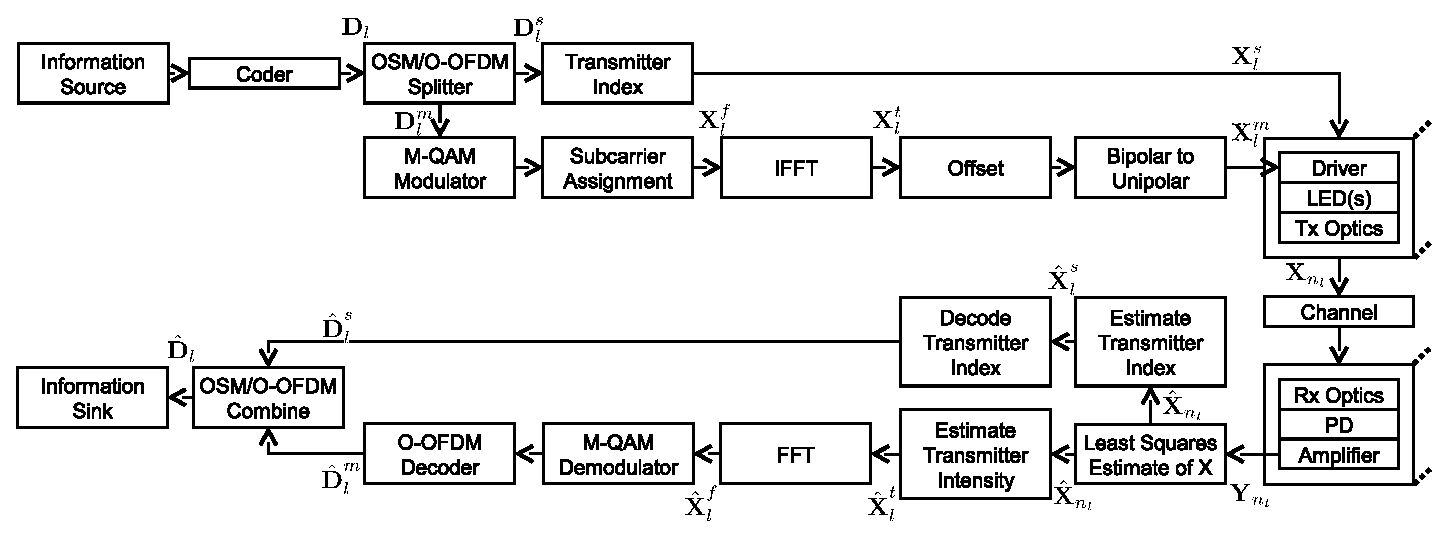
\includegraphics[trim={0.0in 0.0in 0.0in 0.0in}, clip=false, width=6.6in]{figBlockDiagram2.eps}
	%\label{figBlockDiagram}
	\caption{Block diagram of system implementing SIS-OFDM}
\end{figure*}

\newpage
\begin{figure}[htp]
	\centering
		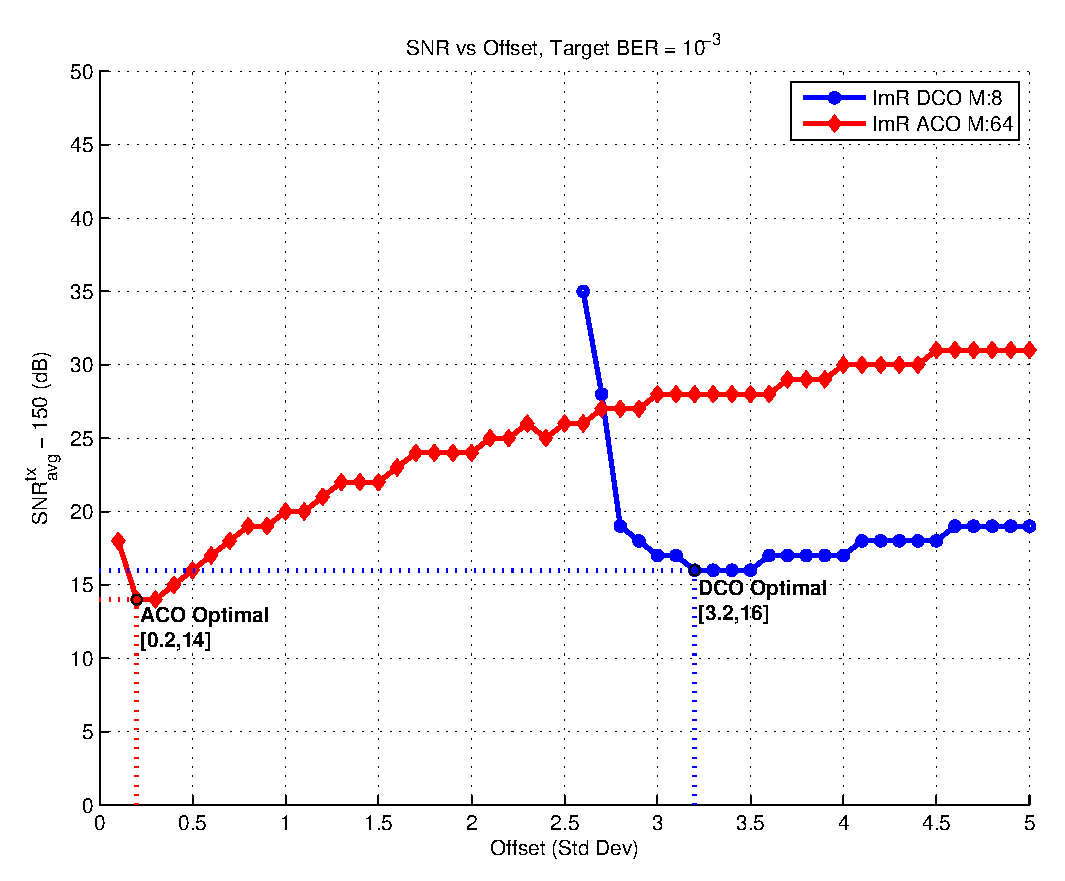
\includegraphics[trim={0.45in 0.25in 0.7in 0.0in}, clip=false, width=5in]{figSNRvsOfst.eps}
	\caption{SNR vs Offset for target BER$= 10^{-3}$ using an ImR}
	%\label{fig:SNRvsOfst}
\end{figure}

\newpage
\begin{figure}[htp]
	\centering
		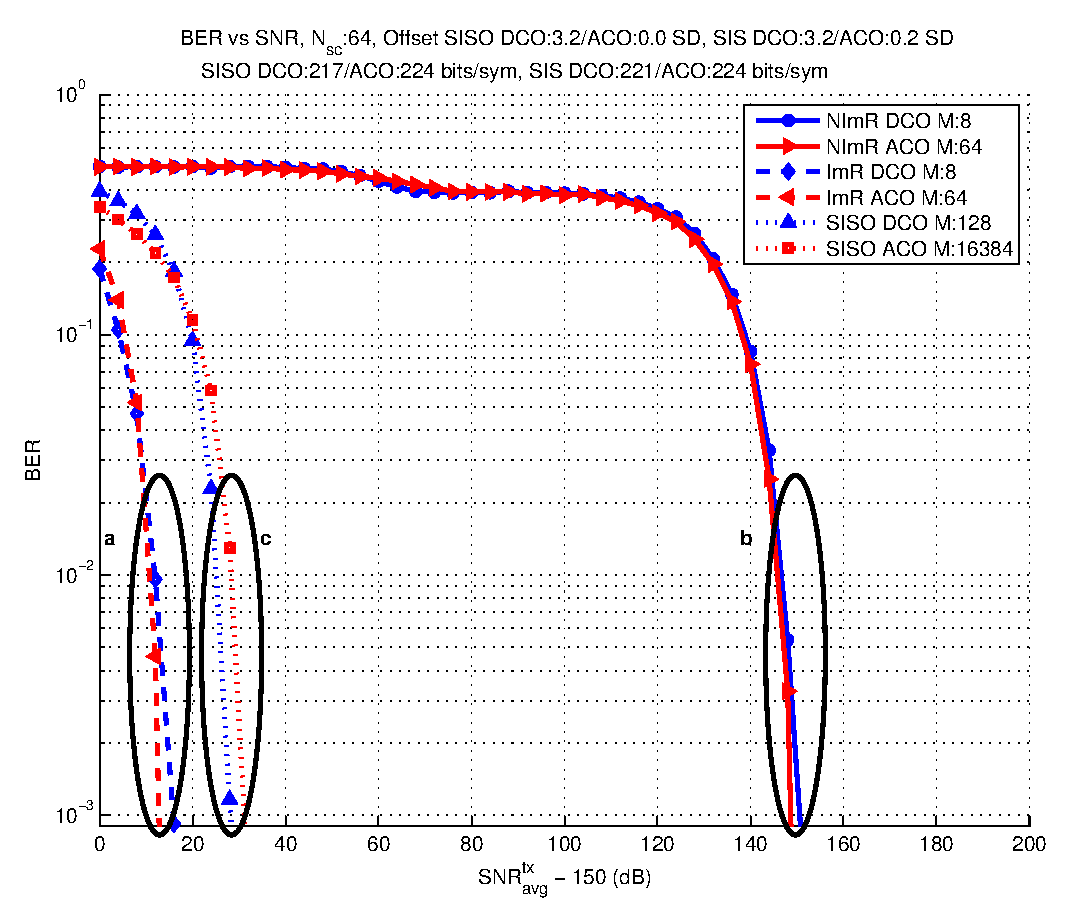
\includegraphics[trim={0.45in 0.15in 0.7in 0.00in}, clip=false, width=5in]{fig_35_64_all.eps}
	\caption{Comparison of BER vs SNR for (a) ImR and (b) NImR}
	%\label{fig:BERnet}
\end{figure}

\newpage
\begin{figure}[htp]
	\centering
		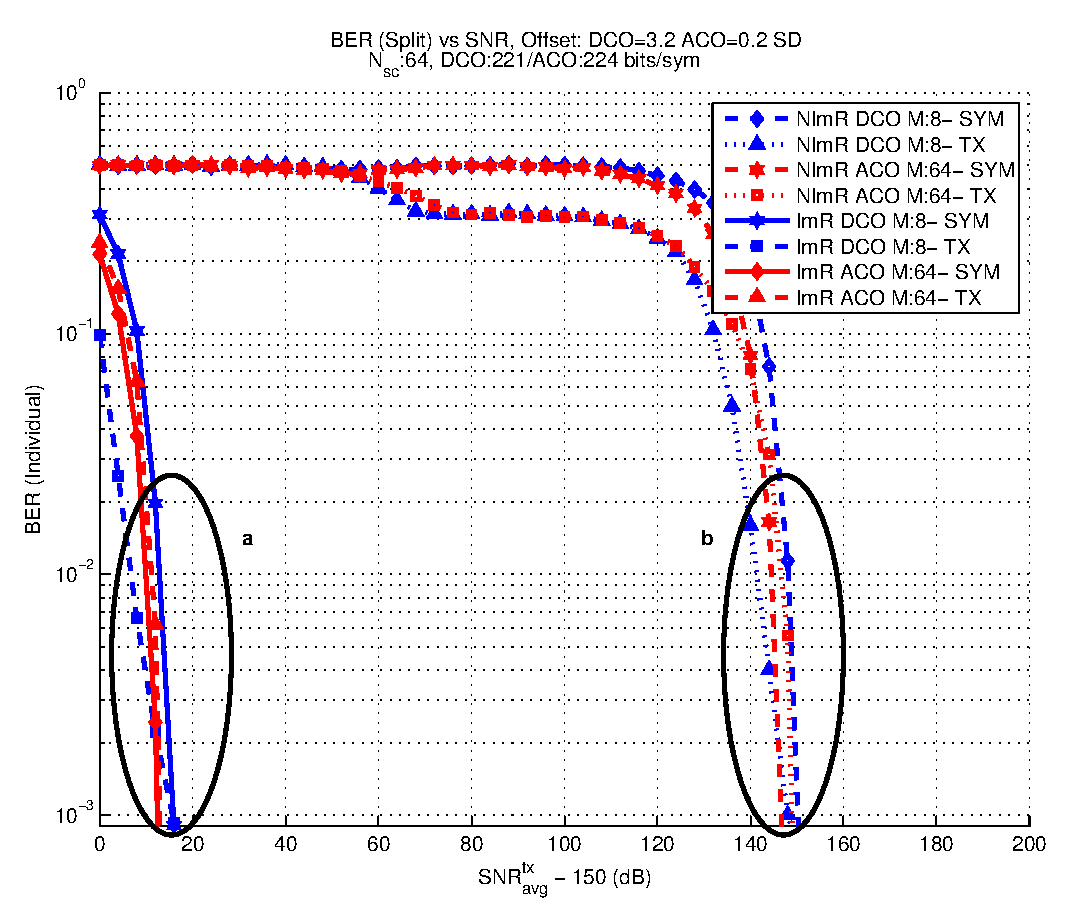
\includegraphics[trim={0.45in 0.15in 0.7in 0.00in}, clip=false, width=5in]{fig_35_64_all_s.eps}
	\caption{Comparison of individual BER vs SNR for (a) ImR and (b) NImR}
	%\label{fig:BERsplit}
\end{figure}

% START ADDING TABLES 
\setcounter{table}{0}
\newpage
\begin{table}[htp]
	\centering
		\begin{tabular}{|c|l|}
			\hline
			{\bf{Stream}}&\multicolumn{1}{|c|}{\bf{Bits}}\\
			\hline
			$\vm{D}_l$ & $\left[\text{ 1 1 0 0 0 1 1 0 0 0 1 1 }\right]^T $\\
			\hline
			$\vm{D}_l^m$ & $\left[\text{ 1 1 0 0 }\right]^T $\\
			\hline
			$\vm{D}_l^s$ & $\left[\text{ 0 1 1 0 0 0 1 1 }\right]^T $\\
			\hline
		\end{tabular}
	\caption{Example SIS-OFDM data streams using ACO-OFDM}
	\label{tabExBits}
\end{table}

\newpage
\begin{table}[htp]
	\centering
      \begin{tabular}{|c|c|c|c|c|c|c|}
			\hline
			{ $n_l$ }&{\bf{OFDM bits}}&$\vm{X}_l^f$&$\vm{X}^t_l$&$\vm{X}^m_l$&{\bf{SM bits}}&$\vm{X}^s_l$\\
			\hline
			0 & - & 0 & 0 & 0 &0 & 1\\
			\hline
			1 & 1 1 & $-1-j$ & $-1$ & 0 &1 & 2\\
			\hline
			2 & - & 0 & $\sqrt{2}$ & $\sqrt{2}$ &1 & 2\\
			\hline
			3 & 0 0 & $1+j$ & $1$ & $1$ & 0& 1\\
			\hline
			4 &-& 0 & 0 & 0 &0 & 1\\
			\hline
			5 &-& $1-j$ & $1$ & $1$ &0 & 1\\
			\hline
			6 &-& 0 & $-\sqrt{2}$ & 0 & 1& 2\\
			\hline
			7 &-& $-1+j$ & $-1$ & 0 &1 & 2\\
			\hline
		\end{tabular}
	\caption{Example subcarrier and luminaire assignment}
	\label{tabExample}
\end{table}

\end{document}
